
%%%%%%%%%%%%%%%%%%%%%%% file typeinst.tex %%%%%%%%%%%%%%%%%%%%%%%%%
%
% This is the LaTeX source for the instructions to authors using
% the LaTeX document class 'llncs.cls' for contributions to
% the Lecture Notes in Computer Sciences series.
% http://www.springer.com/lncs       Springer Heidelberg 2006/05/04
%
% It may be used as a template for your own input - copy it
% to a new file with a new name and use it as the basis
% for your article.
%
% NB: the document class 'llncs' has its own and detailed documentation, see
% ftp://ftp.springer.de/data/pubftp/pub/tex/latex/llncs/latex2e/llncsdoc.pdf
%
%%%%%%%%%%%%%%%%%%%%%%%%%%%%%%%%%%%%%%%%%%%%%%%%%%%%%%%%%%%%%%%%%%%


\documentclass[runningheads,a4paper]{llncs}
\usepackage{amssymb}
\setcounter{tocdepth}{3}
\usepackage[noend]{algpseudocode}
\usepackage{subfig} 
\usepackage{graphicx}
\usepackage{frame, caption}
\usepackage{amsmath}
\usepackage{eulervm}
\usepackage{fontenc}
\usepackage{mathrsfs}
\usepackage{multirow, enumitem, longtable, rotating,lipsum, scrextend}
\usepackage{array}
\usepackage{floatflt}
\usepackage{makecell}
\usepackage{xcolor, soul}
\sethlcolor{yellow}	
\usepackage{floatrow}
\usepackage{setspace}
\newcommand{\argmax}{\operatornamewithlimits{arg\,max}}

\usepackage{url}
\urldef{\mailsa}\path|{alfred.hofmann, ursula.barth, ingrid.haas, frank.holzwarth,|
\urldef{\mailsb}\path|anna.kramer, leonie.kunz, christine.reiss, nicole.sator,|
\urldef{\mailsc}\path|erika.siebert-cole, peter.strasser, lncs}@springer.com|    
\newcommand{\keywords}[1]{\par\addvspace\baselineskip
\noindent\keywordname\enspace\ignorespaces#1}

\begin{document}

\mainmatter  % start of an individual contribution

% first the title is needed
\title{}

% a short form should be given in case it is too long for the running head


% the name(s) of the author(s) follow(s) next
%
% NB: Chinese authors should write their first names(s) in front of
% their surnames. This ensures that the names appear correctly in
% the running heads and the author index.
%
\author{Alfred Hofmann%
%
\and Ursula Barth\and Ingrid Haas\and Frank Holzwarth\and\\
Anna Kramer\and Leonie Kunz\and Christine Rei\ss\and\\
Nicole Sator\and Erika Siebert-Cole\and Peter Stra\ss er}
%

% (feature abused for this document to repeat the title also on left hand pages)

% the affiliations are given next; don't give your e-mail address
% unless you accept that it will be published
\institute{Springer-Verlag, Computer Science Editorial,\\
Tiergartenstr. 17, 69121 Heidelberg, Germany\\
\mailsa\\
\mailsb\\
\mailsc\\
\url{http://www.springer.com/lncs}}

%
% NB: a more complex sample for affiliations and the mapping to the
% corresponding authors can be found in the file "llncs.dem"
% (search for the string "\mainmatter" where a contribution starts).
% "llncs.dem" accompanies the document class "llncs.cls".
%

\toctitle{Lecture Notes in Computer Science}
\tocauthor{Authors' Instructions}
\maketitle


\begin{abstract}
	
 Negotiation has drawn considerable attention in the IA and human-computer interaction fields where several researches proposed efficient decision making models which improves the outcomes of the negotiation. However,negotiation with a human is a process that involves social interaction as well as personal preferences. Indeed, social psychology have provided evidence that social aspects such as interpersonal relation or emotions play an important role in negotiation. For instance, the interpersonal relation of dominance affects the way the negotiators build their strategy of negotiation in term of demand and concessions. This paper present a model of negotiation where the agent is able to express different strategies of negotiation based on its relation of power with the user. The underlying strategies of negotiation are defined from the literature in social psychology. An experiment that studies the effect of the power in the strategy displayed by the agent during its interaction with human participants showed that participants perceived the different strategies of the agent in respect with the power it intended to express. 
 
\end{abstract}


\section{Introduction}
Negotiation as a daily activity in life
interest of building agents that negotiate when defining agents or help to learn negotiation
Social behaviors in negotiation in psychology
proposed implementation 
One important dimension is dominance that we propose to stdy


\section{Model of negotiation based on the relation of power}
	We present a model of \textit{collaborative} negotiation in which an agent and a human user negotiate to reach an agreement, based on each one's \textit{preferences}. In addition, the strategy of negotiation deployed by the agent is based or impacted by the interpersonal relation of power established.
We present in this section the different elements of the collaborative negotiation model based on the relation of power.
\subsection{The negotiation domain}

	The overall goal of the negotiator agent is to reach an agreement about an \textbf{option} in a set of possible options $\mathcal{O}$. 
	Each option is characterized by a set of \textbf{criteria} denoted $\mathcal{C}$. We define for each criterion its domain value $C_i$.
	The set of options $\mathcal{O}$ can be simply defined as the cross-product $C_1\times\ldots\times C_n$ and each option $o\in\mathcal{O}$ is a tuple $(v_1,\ldots,v_n)$, making the simplifying assumption that all options are available. For instance, in a dialogue about restaurants, the criteria might be the type of cuisine and the price, we could have the option: $(French,expensive)$.
	
	\subsubsection{Preference model} 
		We enable the agent to have preferences on each criterion of $\mathcal{C}$, formalized as a set of partial orders $\prec_i$ on each $C_i$. For instance, if the agent prefers affordable restaurants to expenssive, $Expenssive\prec_{Price}Affordable$.
		
		Based on the relation of preferences, we define a function of \emph{satisfaction} that allows the agent to compute whether its like a value or not. Therefore, for a given value $v\in C_i$, the agent computes its \emph{satisfaction} $sat_{self}(v \prec_i)$ for this value as the number of values it prefers less in the partial order $\prec_i$, normalized in [0,1]:
		\vspace{-.5em} 
		\begin{equation}
		sat_{self}(v, \prec_i) =	1 - \left( \frac{|\{v' : v' \neq v \  \wedge \ (v \prec_i v')\}| }{( |C_i| - 1 )}\right)
		\end{equation}
		
	This notion of satisfaction is generalized to any option $o= (v_1, \ldots, v_n)\in \mathcal{O}$ as a simple average
	\vspace{-1em} 
	\begin{equation}
	sat_{self}(o, \prec) = \frac{\sum_{i=1}^{n} sat_{self}(v_i, \prec_i) }{n}
	\vspace{-1.5em} 
	\end{equation}
	

	\subsubsection{Communication model}
	Agent and user communicate through \emph{utterances}. Each utterance type has a specific set of arguments and is associated with a specific expression in natural language (NL). We use five utterance types, based on the work of Sidner \cite{sidner1994artificial} and two additional utterances to close the negotiation (see Table \ref{table:utt}). The NL generation adapts to the discussed topic. The value /$v$/ in Table \ref{table:utt} refers to this NL format to express a value.
	
	
	Each utterance type takes as parameter either a criterion value $v \in C_i$, an option $o \in \mathcal{O}$ or a criterion type $i \in \mathcal{C}$. They can be separated into three groups. 
	
	\begin{itemize}
	\item Information moves (\textit{AskValue/AskCriterion} and \textit{StateValue}) are used to share knowledge about the participant's likings.
	\item Negotiation moves (\textit{Propose}, \textit{Accept} and \textit{Reject}). Throughout the course of the negotiation process, the agent makes offers for both values. Criterion(``Let's go to a Chinese restaurant'') or options (``Let's go to \emph{Chez Francis}''). It has also to respond to offers, by accepting or rejecting them.

	\item Closure moves (\textit{NegotiationSuccess} or \textit{NegotiationFailure}) are used to end the negotiation.
	\end{itemize}
	
	
	%The RejectPropose utterance type is used to clearly reject an option and make a counter-proposal in the same dialogue move. Similarly, the RejectState utterance type is used to make a reject with an explanation. The AcceptPropose is used to accept a criteria and propose a compatible option. 


	\begin{table}[t]
		{\scriptsize
			\begin{tabular} {|p{2.75cm}|p{4cm}|p{3cm}|}
				\hline
				\textbf{Utterance type}  &\textbf{ NL generation} & \textbf{Postcondition}\\
				\hline
				StateValue(v) &  I (don't) like /$v$/. & Speaker : $v \in S_i$ \newline Hearer:  \newline $v\in A_i$ is likable, $v\in U_i$ otherwise \\
				\hline
				AskValue(v)& Do you like /$v$/ ? & \multirow{2}{*}{} \\
				
				AskCriterion(i) &  What kind of /$i$/ do you like ? & \\
				\hline
				ProposeOption(o)  & Let's go to /$o$/. & $o \in P$\\
				
				ProposeValue(v) & Let's go to a /$v$/. & $v \in P_i$\\
				\hline
				AcceptOption(o)& Okay, let's go to /$o$/.& $o \in T$ \\
				
				AcceptValue(v) & Okay, let's go to a /$v$/.& $v \in T_i$ \\
				\hline
				RejectOption(o) & I'd rather choose  something else. & $o \in R$\\
				
				RejectValue(v) &  I'd rather choose  something else. & $v \in R_i$ \\
				\hline
				NegotiationSuccess &  We reached an agreement. & \multirow{2}{*}{}\\
				\cline{1-2}
				NegotiationFailure &  Sorry, but I no longer want to discuss this. & \\
				\hline
				% Counter Propose & $(r,p)\in C_i^2 \vee (r,p) \in \mathcal{O}^2 $ & I don't want to go to $r$. Let's rather go to $p$ \\
				% \hline 
				% RejectState & $x \in \mathcal{O} \vee x\in C_i$ &  I don't like /$x$/, let's choose something else. \\
				% \hline
				% AcceptPropose & $o \in \mathcal{O}$ & Okay. Let's go to /$o$/.\\
				% \hline
			\end{tabular}
		}
		\caption{\label{table:utt}List of utterance types in the model of dialogue.}
	\end{table}
	
	
	\subsection{Dialogue context}
	In order to make cohrent decisions during the negotiation, the agent keeps track of the information shared. 
	\begin{itemize}
		\item \emph{Other statements}: We build the sets $A_i\subseteq C_i$ and $U_i\subseteq C_i$ of values which have been stated by the other as liked or disliked through \emph{StateValue} utterances.
		
		\item \emph{Self statements:} We build the set $S_i \subseteq C_i$ of statements that the agent has made about this criterion which avoids repetition.
		
		\item \emph{Shared proposals:} We define the sets $P$, $T$ and $R$ of respectively open, accepted and rejected proposals in the dialogue.
	
	\end{itemize}

\subsection{the decisional model based on power}

The agent builds its strategy of negotiation with respect to the relation of power its has with the user. Therefore, we initiate the agent with it's belief of power $pow \in [0,1]$. Furthermore, its strategy of negotiation is driven by three main behaviors identified from researches in social psychology. 

	\subsubsection{Level of demand and concessions}
	Dedreu proved in his work \cite{de1995impact} that high-power negotiators show a higher level of demand than the low-power ones. In addition, low-power negotiator's demand decrease over time and the negotiator tends to make larger concessions than high-power negotiators. 
	The notion of concession is implemented by a \emph{concession curve} denoted  $self(pow, t)$ illustrated in figure\ref{fig:conc}
	
		\begin{equation}
		self(pow, t) = \left\{\begin{array}{ll}
		pow & \mathrm{if\ } (t \leq \tau)\\
		max(0, pow - (\frac{\delta}{pow} \cdot (t - \tau))) & \mathrm{otherwise}
		\end{array}\right.
		\end{equation}
		
		\begin{floatingfigure}[r]{1.8in}
			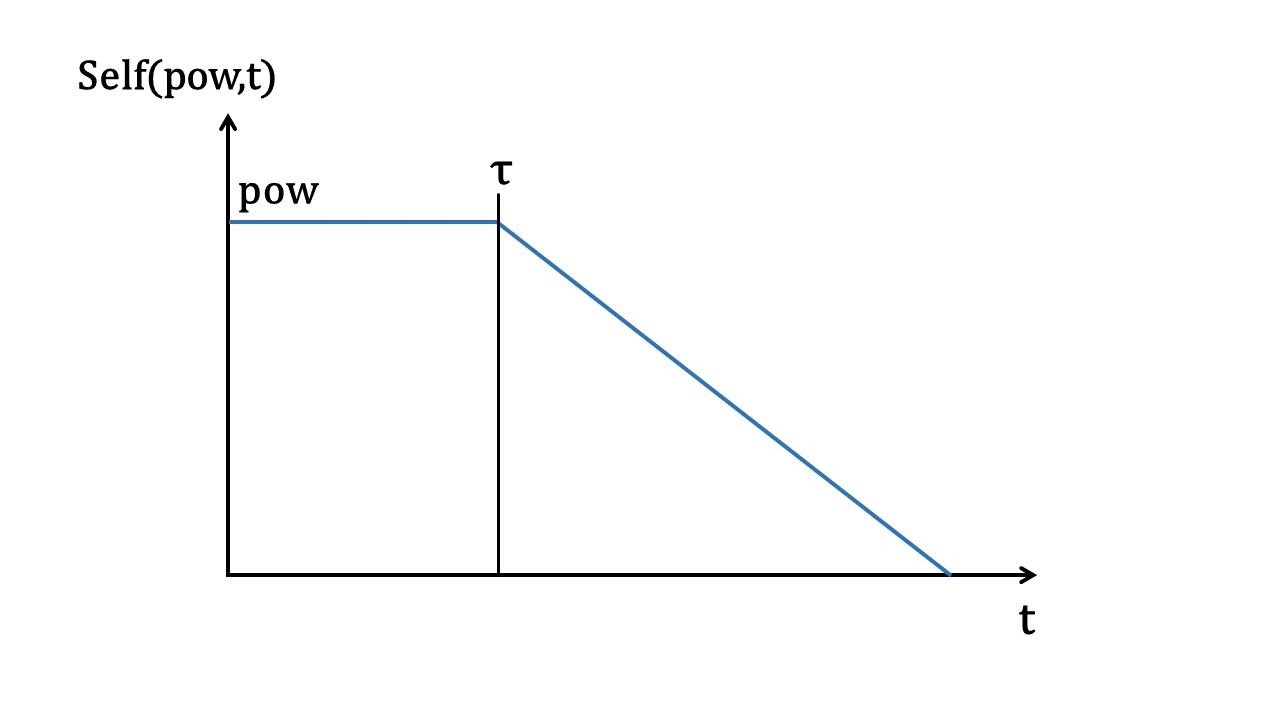
\includegraphics[width=1.8in]{graphs/sv3.png}
			\caption{\label{fig:conc}Concession curve}
		\end{floatingfigure} 
	
	\subsubsection{Self vs other:} Low-power negotiators consider the preferences when making decisions, whereas high-power negotiators are self-centered and only interested in satisfying their own preferences. \cite{fiske1993controlling,de1995impact}
	
	\subsubsection{Controlling the flow of the negotiation:}
	High-power negotiators tend to make the first move \cite{magee2007power} and take the lead in the negotiation. Low-power negotiators aim to construct an accurate model of other preferences, which leads them to ask more questions about other preferences rather than keeping the negotiation going (\emph{e.g} by making proposals)\cite{de2004influence}.
\scriptsize{	
	\bibliographystyle{splncs}
	\bibliography{Library}}
\end{document}
